\subsection{Databus[EK]}
\subsubsection{Allgemein}
Databus ist ein von LinkedIn entwickeltes Tool, welches sich selbst mit den Attributen „source-agnostic distributed change data capture system“ beschreibt. Als Open-Source Software wurde diese im Jahre 2013 unter der Apache-2.0 Lizenz der GitHub-Community bereitgestellt. 
(vgl. \cite{Databus-GitHub})
\vspace{5mm}\par
\textit{Source-Agnostic} bedeutet, dass Databus im Gegensatz zu einer Spezialisierung auf eine bestimmte Datenquelle, wie zum Beispiel ein bestimmter Typus von Datenbanken, darauf ausgelegt ist, ein breitgefächertes Spektrum an Datenquellen abzudecken. Damit soll die Unabhängigkeit von den Datenquellen gewährleistet werden.
\vspace{5mm}\par
\textit{Distributed} heißt, dass es sich bei Databus um ein verteiltes System handelt, welches sich die Vorteile von mehreren Computersystem zu Nutze machen kann und somit nicht auf ein singuläres System angewiesen ist.
\vspace{5mm}\par
\textit{Change-Data-Capture} (CDC) beschreibt einen Prozess, bei welchem die Änderung in einer Datenquelle - oft einer Datenbank - identifiziert und festgehalten wird. Diese gewonnen Änderungen werden dann an andere Systemarchitekturen, wie zum Beispiel ETL-Prozessen, zur Weiterverarbeitung zur Verfügung gestellt.
(vgl. \cite{CDC})
\newpage
\subsubsection{Wie funktioniert Databus?}
\begin{figure}[H]
    \centering
    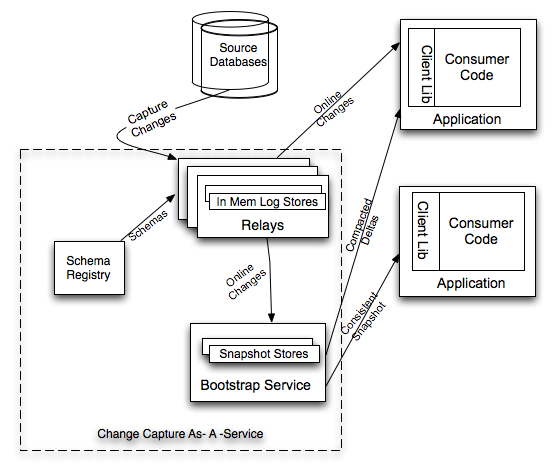
\includegraphics[scale=0.4]{images/databus-as-a-service.png}
    \caption{Databus-Aufbau (02.04.2020)}
    \label{img:}
    \url{http://s3.amazonaws.com/snaprojects/databus/databus-as-a-service.png}
\end{figure}
Wie man in der oben aufgezeigten Grafik sehen kann, besteht Databus aus folgenden drei Teilen: 
\begin{enumerate}
  \item \textbf{Relais:} Nimmt die aufgezeichneten Änderungen in der Datenquelle entgegen. Diese Änderungen werden in einem in-memory Log-Store abgespeichert, da dieser über die nötigen high-performance Eigenschaften verfügt.
  \item \textbf{Bootstrap-Service:} Periodisch nimmt dieser Daten des Relais entgegen. Ermöglicht wird dies durch eine periodische Umlenkung des Relais-Datenstroms auf den Bootstrap-Service. Dieser Service speichert die erhaltenen Daten dann als sogenannten Snapshot - eine Momentaufnahme der Daten zu einem bestimmten Zeitpunkt - ab.
  \item \textbf{Client-Library:} Diese wird in die Applikation eingefügt, um Daten aus dem Relais oder Bootstrap-Service erhalten zu können.
\end{enumerate}
Sollte der Fall eintreten, dass ein Consumer - eine Applikation, welche die Client-Library verwendet - datentechnisch zeitlich zurückfällt, so dass die benötigten Daten im Relais nicht länger vorliegen, kommt es zu folgendem Fall: ein konsolidierter Snapshot wird dem zurückliegenden Consumer übergeben, welcher diesen wieder auf Kurs bringt. Ähnlich sieht der Fall aus, wenn sich einer neuer Consumer einklinkt. Der Bootstrap-Service stellt auch in diesem Fall einen Snapshot bereit, welcher es dem Consumer ermöglicht, auf den aktuellen Stand zu kommen.
(vgl. \cite{Databus-Open-Sourcing})
\subsubsection{Entscheidungsprozess}
In der ersten Phase der Arbeit, sozusagen der Aneignungsphase, war Databus noch im Technologie-Stack enthalten. Anfangs wirkte das Tool vielversprechend für die Firma, durch Aspekte wie die freie Verfügbarkeit als Open-Source Software und damit die Möglichkeit eines Einblicks in dessen Funktionsweise. Doch bei weiterer Einarbeitung und Kenntnisnahme über die genaue Funktionalität, wurde die Verwendung von Databus auf Eis gelegt. Für die Firma MIC ist die Tatsache, dass man für die Verwendung von Databus jede Tabelle, welche auf Änderung beobachtet wird, abändern muss, ein Problem. Der Grund dafür liegt an der Menge der Tabellen, welche abgeändert werden müssten und dass ein solches Vorgehen nicht dem Echtzeitbetrieb vereinbar ist.

\subsubsection{Die Problematik verwahrloster Open-Source Software}
Wenn eine zuvor intern in Unternehmen entwickelte Software den Schritt macht, in den Open-Source Bereich entlassen zu werden, dann oft mit der Hoffnung, durch größere Beteiligung der Community und auch anderer Unternehmungen am Ende eine bessere Software zu erhalten, als wenn diese inhouse entwickelt worden wäre.
\vspace{5mm}\par
Dies beschreibt allerdings nur den Optimalfall. Durch die schnellen Veränderungen in einer Branche wie dieser kann es schnell zu Problemen bei der Nutzbarkeit der Software kommen, wenn diese nicht regelmäßig gewartet wird.So auch der Fall bei Databus, selbst die Replikation der auf GitHub präsentierten Beispiele war nur durch externe fremdsprachige Ressourcen möglich. Somit ist ein deutlich größerer Zeitaufwand  nötig, welcher nur schwer im voraus zu kalkulieren ist. Ohne also eine große Code-Kenntnis der Software kann ein solches Unterfangen schnell zu einer Gefahr werden, wenn längerfristig Projekte darauf aufgebaut werden sollen. 
\newpage
\subsection{Kafka[EK]}
\begin{figure}[H]
    \centering
    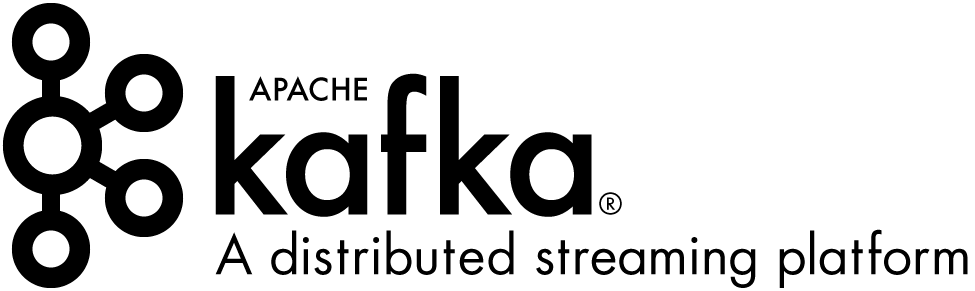
\includegraphics[scale=0.4]{images/kafka_logo.png}
    \caption{Kafka Logo (02.04.2020)}
    \url{https://kafka.apache.org/images/logo.png}
\end{figure}
\subsubsection{Allgemein}
Bei Kafka handelt es sich um eine verteilte Streaming-Plattform, welche von LinkedIn im Jahre 2011 als Open-Source Projekt veröffentlicht wurde. 
(vgl. \cite{Kafka-Open-Sourcing})Durch den Apache Incubator kam das Projekt im Jahre 2012 in die Hände der Apache Software Foundation und wird seitdem auch von Apache weiterentwickelt und gewartet.
(vgl. \cite{Kafka-Apache-Incubator})
\vspace{5mm}\par
Als Streaming-Plattform deckt Kafka drei Funktionalitäten ab.
Erste wäre das Ver-öffentlichen und Abonnieren von Record-Streams (Kafkas Bezeichnung für einen Datenstrom), ähnlich zu einem Enterprise-Messaging-System (EMS). Zweite wäre das Speichern von solchen Record-Streams, in einer Weise, in welcher diese dauerhaft fehlertolerant erfolgen. Dritte wäre die Verarbeitung von Streams im Moment des Auftretens.
\vspace{5mm}
Kafka soll vor allem diesen zwei Klassen von Applikationen zur Seite stehen:
\begin{itemize}
    \item Echtzeit Streaming-Data-Pipelines, welche zuverlässig Daten zwischen System oder auch Applikationen transportieren.
    \item Echtzeit Streaming-Applikationen, welche auf Daten-Streams reagieren oder diese transformieren.
\end{itemize}
(vgl. \cite{Kafka-Introduction})

\subsubsection{Wie funktioniert Kafka?}
Kafka wird als ein sogenannter Cluster auf einem oder mehreren Servern ausgeführt. 
\vspace{5mm}\par
Ein Cluster ist: „Eine Gruppe von unabhängigen Servern (üblicherweise in unmittelbarer Nähe zu einander), welche durch ein dediziertes Netzwerk vernetzt als eine zentralisierte Datenverarbeitungsressource arbeiten“
\cite{Cluster-Definition}
\newpage
Dieser Cluster speichert dann die Record-Streams in sogenannten Topics - die Kategorien für die Aufzeichnungen. Jede dieser Aufzeichnungen beziehungsweise Records steht aus dreierlei Bestandteilen: dem Key (eindeutige Identifikation), dem dazugehörigen Value (Wert) und einem Zeitstempel. Für das Management dieser Cluster verwendet Kafka Zookeeper.
\begin{figure}[H]
    \centering
    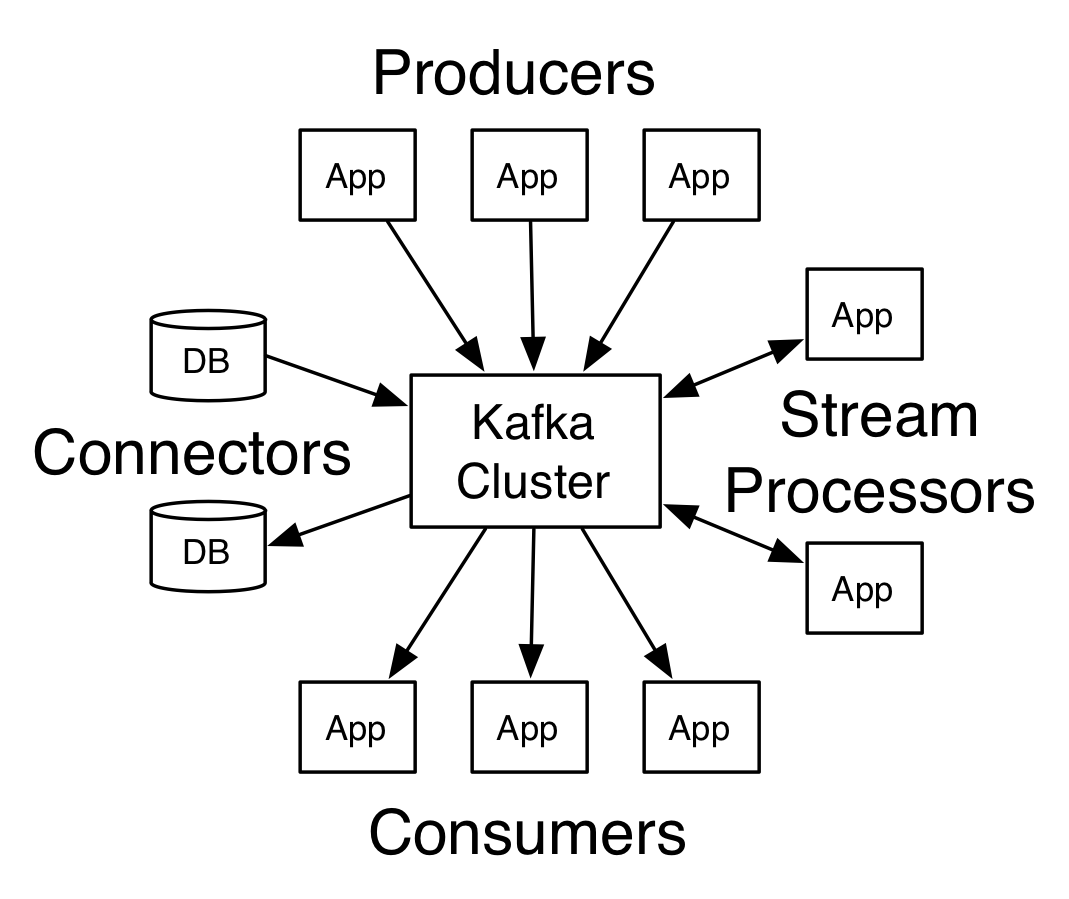
\includegraphics[scale=1.5]{images/kafka-apis.png}
    \caption{Kafka APIs (02.04.2020)}
    \url{https://kafka.apache.org/23/images/kafka-apis.png}
\end{figure}
Wie in der vorhergehenden Grafik zu sehen ist, bilden vier Core-APIs Kafka:
\begin{enumerate}
  \item \textbf{Producer API:} Will eine Applikation einen Record-Stream an den Kafka-Cluster und damit an ein Topic senden, so kann sie dies über diese API lösen.
  \item \textbf{Consumer API:} Bildet das Gegenstück zur Producer API; will eine Applikation zu einem bestimmten Topic zugehörige gesendete Record-Streams haben, muss jene einfach dieses Topic abonnieren.
  \item \textbf{Stream API: } Nimmt die beiden vorangegangen API-Funktionen Eins und Zwei an. Somit kann eine Applikation als ein Stream-Prozessor agieren, welcher sowohl den Input-Stream eines Topics konsumiert, als auch den Output-Stream zu einem anderen Topic liefert. So kann diese API einen Input-Stream zu einem Output-Stream transformieren.
  \item \textbf{Connector API:} Soll die Möglichkeit, geben bereits vorhanden Systeme und Applikationen mit einem Kafka-Topic zu verbinden, dies kann einerseits als Consumer und andererseits auch als Producer erfolgen. Ein Beispiel für einen Producer  wäre, wenn jede Änderung einer Datenbanktabelle aufgezeichnet werden soll und über den Kafka-Cluster für eine Weiterverarbeitung bereitstehen soll.
\end{enumerate}
Die APIs erlauben darüber hinaus, nicht nur die Verarbeitung eines Topics. Alle beschriebenen Funktionalitäten sind auch mit mehreren Topics möglich.
(vgl. \cite{Kafka-Introduction})
\subsubsection{Entscheidungsprozess}
Die Echtzeit-Komponente von Kafka ist ein tragender Grund für die Verwendung in dieser Arbeit, dies ermöglicht den Komponenten ohne größeren Zeitverlust die weiterzugebenden Daten mit der nachfolgenden Komponente zu kommunizieren. Des weiteren handelte es sich bei Kafka um eine Vorgabe der Firma MIC.

\subsection{ZooKeeper[EK]}
\begin{figure}[H]
    \centering
    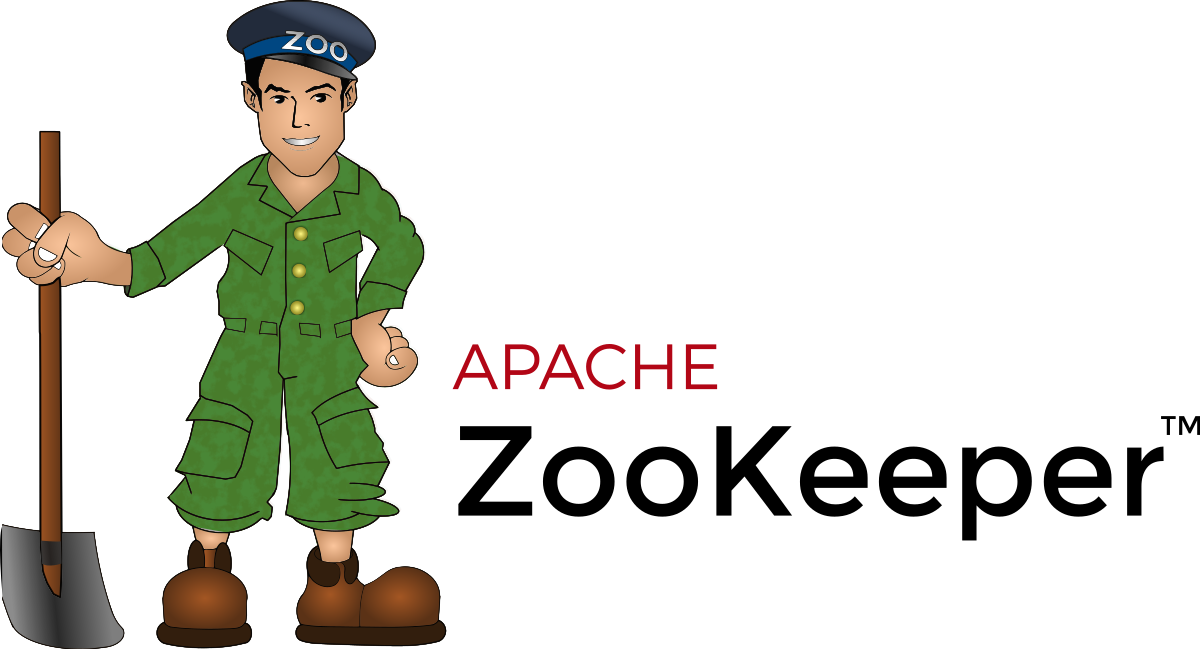
\includegraphics[scale=0.25]{images/zookeeper-logo.png}
    \caption{ZooKeeper Logo (02.04.2020)}
    \url{https://upload.wikimedia.org/wikipedia/en/thumb/8/81/Apache_ZooKeeper_Logo.svg/403px-Apache_ZooKeeper_Logo.svg.png}
\end{figure}
\subsubsection{Allgemein}
ZooKeeper ist eine Open-Source Software, welche von Freiwilligen unter dem Dach der Apache Software Foundation entwickelt wird. Ziel des Projektes ist es, einen Server, der eine sehr zuverlässige Koordination von verteilten System ermöglicht, bereitzustellen. 
(vgl. \cite{Apache-ZooKeeper})
\subsubsection{Nutzen für Kafka}
Beim Management der Cluster für Kafka fallen die folgenden Aufgaben an ZooKeeper. Die Koordinierung von Brokern. Das Bereitstellen von einem konsistenten Dateisystems für die Konfigurationsdateien. Die Auswahl eines sogenannten „Broker Topic Partition Leaders”.
(vgl. \cite{Kafka-Architecture})

\subsubsection{Funktionsweise}
Die interne Datenstruktur von ZooKeeper ähnelt einem Baum, heißt von dem Ausgangspunkt beziehungsweise der Wurzel erreichen wir alle weiteren Elemente über eine direkte Verbindung oder über deren übergeordneten Elemente. Jedes Element in diesem Baum ist ein Knoten, eine sogenannte zNode (z steht für Zookeeper, Node ist der englische Begriff für Knoten). Ein Beispiel dafür ist in der folgenden Grafik zu sehen.
\begin{figure}[H]
    \centering
    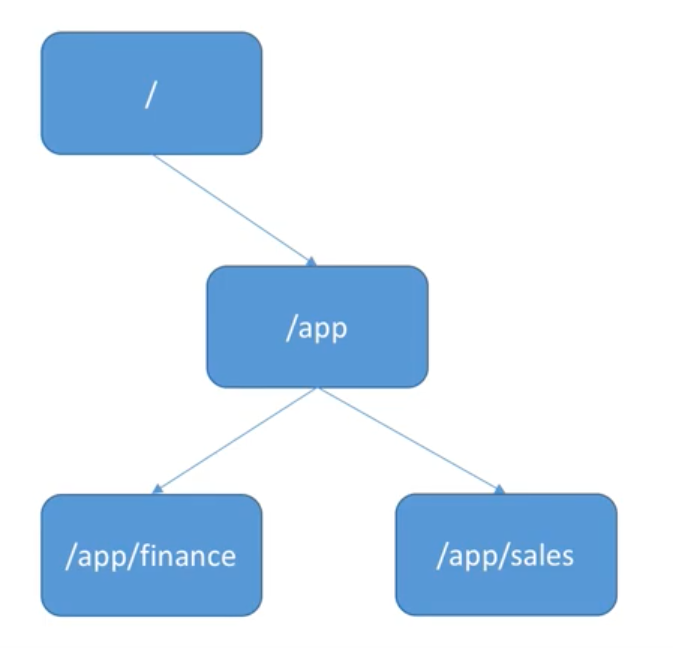
\includegraphics[scale=0.3]{images/zookeeper-node.png}
    \caption{ZooKeeper zNodes (02.04.2020)}
    \url{https://youtu.be/AS5a91DOmks?t=161}
    \label{img:}
\end{figure}
Die Eigenschaften einer zNode sind, dass jede über einen Pfad verfügt und entweder persistent oder ephermal sein kann - Kafka verwendet beide. Mit persistent ist gemeint, dass die zNode immer existiert, also somit eine persistente Präsenz aufweist. Die ephemeral zNode ist nur zur Zeit der Verbindung mit der Applikation existent. Darüber hinaus kann eine zNode Daten speichern, kann nicht umbenannt werden und bietet die Möglichkeit für eine Observierung. Heißt, dass sich Abonnenten dieser zNode darüber informieren lassen können, ob eine Änderung in dieser stattgefunden hat.
(vgl. \cite{ZooKeeper-Video})
\subsubsection{Entscheidungsprozess}
Als ein Bestandteil von Kafka, fällt eine jede direkte Entscheidung weg, da eine Entscheidung für Kafka immer auch eine für Zookeeper ist.

\subsection{Kotlin[EK]}
\begin{figure}[H]
    \centering
    
\includegraphics[scale=0.1]{images/kotlin-logo.png}
    \caption{Kotlin Logo (02.04.2020)}
    \url{https://upload.wikimedia.org/wikipedia/commons/thumb/7/74/Kotlin-logo.svg/1024px-Kotlin-logo.svg.png}
\end{figure}
\subsubsection{Allgemein}
Bei Kotlin handelt es sich um eine relativ neue Sprache, welche im Jahre 2011 von JetBrains ins Leben gerufen wurde. Als Open-Source Sprache ist diese nicht allein von JetBrains abhängig, seit Google sie im Jahre 2017 als die neue offizielle Sprache für Android über Java ernannt hat. Folgend stiegen auch sie bei der Entwicklung ein. Darüber hinaus, wie bei den meisten Open-Source Projekten, beteiligt sich auch die Community an der Entwicklung der Sprache. Ziel der Sprache ist die Multiplattform. Kotlin-Code ist damit nicht nur auf der JVM lauffähig, sondern auch Native und im Web. Gemeinsam bilden Google und JetBrains die Kotlin Foundation.
\subsubsection{Merkmale}
\begin{itemize}
  \item \textit{Kurz und prägnant.} Ein sogenanntes POJO mit Gettern, Settern und Standardfunktionen, wie „toString()“ können in einer Zeile geschrieben werden. Lamda-Expressions erlauben Operationen, wie zum Beispiel das Filtern einer Liste, ohne viel Boilerplate-Code. 
  \item  \textit{Typsicherheit und keine NullPointer-Exceptions.} Kotlin ist eine stark und statisch typisierte Programmiersprache. Eine Variable für den Compiler darf nicht den Wert null annehmen, außer dies wird explizit angegeben. Bei einer Typenprüfung wird die Variable automatisch gecastet und erlaubt somit den direkten Zugriff auf die typenspezifischen Felder, Eigenschaften und Funktionen.
  \item  \textit{Interoperabel.} Kotlin kann, je nach Target-Plattform, auf die existierenden Öko-systeme zugreifen. So kann in der JVM-Plattform die große Vielfalt an existierenden Libraries genutzt werden.
\end{itemize}
(vgl. \cite{Kotlin-Lang})
\subsubsection{Syntax}
Da in Kontext dieses Projekts Kotlin vor allem als Ersatz für Java eingesetzt wird, wird hier die Syntax im Vergleich zu Java erläutert. Dies heißt, das auf Unterschiede eingegangen wird, welche vor allem der Veranschaulichung der Argumentation für den Entscheidungsprozess dienen soll.
\begin{lstlisting}[caption={Kotlin-Hello-World}, language=Kotlin]
fun main() {
    println("Hello world!")
}
\end{lstlisting}
\vspace{4mm}\par
Wie auch in Java ist die Main-Funktion der Einstiegspunkt der Applikation. Bereits jetzt wird im Beispiel ersichtlich, dass mit deutlich weniger Zeilen das klassische Hello-World-Programm geschrieben werden kann. In Kotlin darf auf die in Java obligatorische Klasse verzichtet werden; Funktionen werden im Unterschied mit dem Kürzel „fun“ deklariert. Es entfallen auch die Einstiegsargumente, welche bei Bedarf jedoch angegeben und verwendet werden können. Es entfällt in den meistens Fällen auch das Semikolon „;“. 
Hier der gleiche Code in Java:
\begin{lstlisting}[caption={Java-Hello-World}, language=Kotlin]
class HelloWorld {
    public static void main(String[] args) {
        System.out.println("Hello, World!"); 
    }
}
\end{lstlisting}
\vspace{4mm}\par
Im Bereich der Variablen bietet Kotlin alle bereits bekannten Datentypen, auch gibt es die Möglichkeit spezielle Datentypen über Java-Libraries zu nutzen. Im Unterschied zu Java muss der Datentyp nicht zwingend angeben werden, wenn der Compiler dies aus dem Kontext lesen kann. Hier die Möglichkeiten eine Variable zu deklarieren:
\vspace{3mm}\par
\newpage 
\begin{lstlisting}[caption={Val \& Var}, language=Kotlin]
val a: Int = 1
val b = 2
val c: Int 
var d = 3
\end{lstlisting}
\vspace{4mm}\par
An erster Stelle der Deklaration gibt die Art der Variable an, dies kann val oder var  sein. Val definiert eine read-only Variable. Bei Var hingegen handelt es sich um ein Variable, welche jederzeit, konform nach ihrem Datentyp, neu zugeordnet werden kann. 
Beim Wert c können wir sehen, dass der Compiler zu dieser Zeit noch nicht wissen kann, um welchen Datentyp es sich handelt, aus diesem Grund muss dieser explizit angegeben werden.
Eine weitere Besonderheit von Kotlin ist, dass ein „if“ auch als Expression fungieren kann, dies sieht wie folgt aus:
\vspace{3mm}\par
\begin{lstlisting}[caption={if-Expression}, language=Kotlin]
c = if (a > b) a else b
\end{lstlisting}
\vspace{4mm}\par
Hiermit wird immer die größere Zahl von a und b auf c zugewiesen.
(vgl. \cite{Kotlin-Basic-Syntax})
\subsubsection{Entscheidungsprozess}
Die Möglichkeiten wären Java, Python und Kotlin gewesen. Kotlin wurde als Sprache gewählt, da vor allem die schnelle Entwicklung von den Eigenschaften, wie weniger Boilerplate und dem Wegfallen der Nullpointer-Exceptions, profitiert. Dies sind aber vor allem persönliche Präferenzen, welche auch mit anderen Sprachen hätten erreicht werden können. Schlagkräftiges Argument war die Interoperabilität mit Java, da die Firma auf einer großen Java-Codebase sitzt. Wissen von Java kann daher schnell in Kotlin angewandt werden. Die Kompaktheit des Codes in Kotlin und der Möglichkeit auf Java-Code und deren Libraries zurückzugreifen unterstützte die Wahl.
